\chapter{Arhitektura i dizajn sustava}

\noindent Arhitekturu sustava dijelimo na tri različita dijela: \textbf{frontend}, \textbf{backend} i \textbf{bazu podataka}. Jedino koordinirana implementacija ovih podsustava zajedno dovodi do kvalitetnog finalnog proizvoda u obliku web platforme koju ostvarujemo. 
\newline \newline
\noindent \textbf{\textit{Frontend}} predstavlja sučelje između korisnika i same platforme. Konkretno, on pruža korisniku pregled sadržaja web stranice i omogućava mu komunikaciju s aplikacijom putem \textit{HTTP} (\textit{HyperText Transfer Protocol}) zahtjeva. Frontend je implementiran uz pomoć \textit{JavaScripta} (radnog okvira \textit{React.js}), \textit{HTML-a} i \textit{CSS-}a.
\newline\newline\noindent \textbf{\textit{Backend}} je taj koji te \textit{HTTP} zahtjeve obrađuje i upravlja podatcima u bazi podataka. Neke od funkcionalnosti koje omogućuje backend su primjerice registracija novog korisnika ili brisanje korisnika od strane sistemskog administratora. \textbf{Controller - Service - Repository} troslojna arhitektura temelj je backend implementacije aplikacije. \textit{Controller} sloj povezuje frontend i backend, pozivajući \textit{Service} sloj da obradi zahtjeve korisnika. Ako je za obradu tih zahtjeva potreban pristup bazi podataka, \textit{Service} sloj poziva funkcije \textit{Repository} sloja koji to omogućuje. Za ostvaranje backenda korišten je programski jezik \textit{Java} (radni okvir \textit{Spring Boot}), a odabrana je razvojna okolina \textit{Intellij IDEA}. Ispitivanje backend funkcionalnosti omogućeno je korištenjem \textit{Postman} platforme.
\newline\newline\noindent \textbf{\textit{Baza podataka}} spremište je entiteta koji su prikazani u obliku tablica s atributima. Iz nje se često čitaju, u nju dodaju i po potrebi u njoj ažuriraju podatci. Kritičan je dio arhitekture sustava. Baza podataka izgrađena je korištenjem \textit{PostgreSQL} sustava za upravljanje bazom podataka.

			\begin{figure}[H]
			    \centering
			    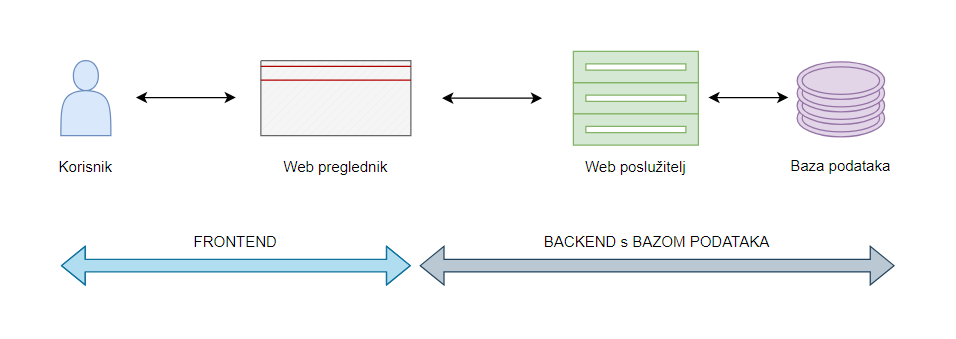
\includegraphics[width=1\linewidth]{slike/skica_arhitekture.png}
			    \caption{Skica arhitekture sustava}
			    \label{fig:enter-label}
			\end{figure}
   
\bigskip
   
   			\begin{figure}[H]
			    \centering
			    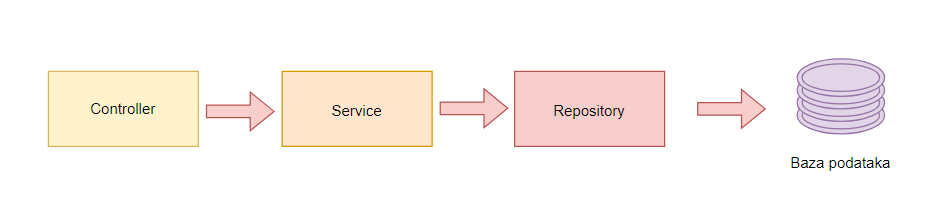
\includegraphics[width=1\linewidth]{slike/csr_arh.png}
			    \caption{Skica \textbf{Controller - Service - Repository} troslojne arhitekture backenda}
			    \label{fig:enter-label}
			\end{figure}

   \eject

		\section{Baza podataka}
			
		Za našu platformu koristit ćemo relacijsku bazu podataka. Objekt takve baze je relacija, odnosno tablica koja je definirana svojim imenom i skupom atributa. Atributi unutar jednog entiteta mogu poprimiti funkciju primarnog ili stranog ključa.
Baza podataka u našem se slučaju sastoji se od 5 entiteta - \textbf{profile}, \textbf{recipe}, \textbf{follow}, \textbf{likes} i \textbf{comment}.
		
			\subsection{Opis tablica}

\noindent \textbf{\textit{profile}}\\
\begin{samepage}
Ovaj entitet sadrži osnovne informacije o korisničkom profilu i  sastoji se od sljedećih atributa: \textit{userID} (autogenerirani identifikator korisnika), \textit{email }(e-mail adresa), \textit{username} (korisničko ime), \textit{password} (lozinka), \textit{name} (ime), \textit{surname} (prezime) i \textit{age} (dob). Atribut\textit{ userID} primarni je ključ entiteta \textbf{profile}. 
\end{samepage}

    				\begin{longtblr}[
					label=none,
					entry=none
					]{
						width = \textwidth,
						colspec={|X[6,l]|X[6, l]|X[20, l]|}, 
						rowhead = 1,
					} %definicija širine tablice, širine stupaca, poravnanje i broja redaka naslova tablice
     
					\hline \SetCell[c=3]{c}{\textbf{profile}}	 \\ \hline[3pt]
					\SetCell{LightGreen}userID & VARCHAR	&  	jedinstveni identifikator korisnika	\\ \hline
					\SetCell{}email & VARCHAR	&  	jedinstvena e-mail adresa korisnika 	\\ \hline
					\SetCell{} name & VARCHAR	&  ime korisnika (opcionalno)	\\ \hline
					\SetCell{} surname & VARCHAR	&  	prezime korisnika (opcionalno)	\\ \hline
					\SetCell{} age & INT	&  	dob korisnika (opcionalno)	\\ \hline
					\SetCell{} password & VARCHAR	&  lozinka korisnika 	\\ \hline
					\SetCell{}username & VARCHAR	&  	jedinstveno korisničko ime	\\ \hline
               		
                    
                    
				\end{longtblr}

    
\noindent \textbf{\textit{recipe}}\\
\begin{samepage}
Ovaj entitet opisuje recept postavljen na platformu od strane registriranog korisnika. Primarni je ključ entiteta \textit{recipeID} (autogenerirani identifikator recepta), a strani ključ \textit{userID} koji povezuje entitete \textbf{recipe} i \textbf{profile}.
\end{samepage}

\begin{samepage}
\noindent Ostali atributi su: \textit{ingredients} (sastojci jela koje recept opisuje), \textit{name} (ime recepta), \textit{instructions} (niz uputa pripreme jela opisanog receptom), \textit{origin} (mjesto podrijetla jela), \textit{category} (kategorija jela), \textit{specialTag} (dodatne oznake), \textit{imageURL} (URL slike koju korisnik prilaže uz postavljeni recept), \textit{videoURL} (URL videa koji korisnik prilaže uz postavljeni recept) te \textit{preparationTime} (vrijeme potrebno za spremanje receptnog jela).
\end{samepage}
    
    				\begin{longtblr}[
					label=none,
					entry=none
					]{
						width = \textwidth,
						colspec={|X[8, l]|X[6, l]|X[20, l]|}, 
						rowhead = 1,
					} %definicija širine tablice, širine stupaca, poravnanje i broja redaka naslova tablice
					\hline \SetCell[c=3]{c}{\textbf{recipe}}	 \\ \hline[3pt]
					\SetCell{LightGreen}recipeID & VARCHAR	&  	jedinstveni identifikator recepta 	\\ \hline
                    \SetCell{} ingredients & VARCHAR	&  	popis sastojaka receptnog jela 	\\ \hline
                    \SetCell{} name & VARCHAR	&  	ime recepta 	\\ \hline
                    \SetCell{} instructions & VARCHAR	&  	niz uputa za pripremu jela prema receptu 	\\ \hline
                    \SetCell{} origin & VARCHAR	&  	mjesto podrijetla receptnog jela (opcionalno)	\\ \hline
                    \SetCell{} category & VARCHAR	&  	vrsta (kategorija) receptnog jela	\\ \hline
                    \SetCell{} specialTag & VARCHAR	&  	specijalne dodatne oznake receptnog jela (opcionalno)	\\ \hline
                    \SetCell{} videoURL & VARCHAR	&  	URL videa priloženog uz recept (opcionalno)	\\ \hline
					\SetCell{} imageURL & VARCHAR	&  	URL slike priložene uz recept 	\\ \hline
    				\SetCell{} preparationTime & INT	&  	vrijeme kuhanja jela u minutama	\\ \hline
					\SetCell{LightBlue}userID & VARCHAR	&  	jedinstveni identifikator korisnika 	\\ \hline
				\end{longtblr}
				\noindent \textbf{\textit{follow}}\\
\begin{samepage}
Ovaj entitet predstavlja vezu koja se stvara između 2 korisnika kada dođe do praćenja i  sastoji se od sljedećih atributa: \textit{userID} i \textit{followerId} koji u paru čine primarni ključ relacije, a oba su također i strani ključevi uzeti iz relacije \textbf{profile}.
\end{samepage}

    				\begin{longtblr}[
					label=none,
					entry=none
					]{
						width = \textwidth,
						colspec={|X[6,l]|X[6, l]|X[20, l]|}, 
						rowhead = 1,
					} %definicija širine tablice, širine stupaca, poravnanje i broja redaka naslova tablice
     
					\hline \SetCell[c=3]{c}{\textbf{follow}}	 \\ \hline[3pt]
					\SetCell{LightGreen}userID & VARCHAR	&  	jedinstveni identifikator korisnika	\\ \hline
					\SetCell{LightGreen}followerId & VARCHAR	&  	jedinstveni identifikator korisnika 	\\ \hline
					
                    
                    
				\end{longtblr}
				\noindent \textbf{\textit{likes}}\\
\begin{samepage}
Ovaj entitet predstavlja vezu koja se stvara prilikom označavanja recepata i  sastoji se od sljedećih atributa: \textit{userID} i \textit{recipeId} koji u paru čine primarni ključ relacije, a oba su također i strani ključevi uzeti iz relacija \textbf{profile} i \textbf{recipe}
\end{samepage}

    				\begin{longtblr}[
					label=none,
					entry=none
					]{
						width = \textwidth,
						colspec={|X[6,l]|X[6, l]|X[20, l]|}, 
						rowhead = 1,
					} %definicija širine tablice, širine stupaca, poravnanje i broja redaka naslova tablice
     
					\hline \SetCell[c=3]{c}{\textbf{likes}}	 \\ \hline[3pt]
					\SetCell{LightGreen}userID & VARCHAR	&  	jedinstveni identifikator korisnika	\\ \hline
					\SetCell{LightGreen}recipeId & VARCHAR	&  	jedinstveni identifikator recepta	\\ \hline
					
                    
                    
				\end{longtblr}
				\noindent \textbf{\textit{comment}}\\
\begin{samepage}
Ovaj entitet sadrži osnovne informacije o komentarima i sastoji se od sljedećih atributa: \textit{userID}, \textit{recipeId}, \textit{timestamp} (vremenska oznaka komentara) i \textit{text} (tekst komentara). Atributi \textit{userId} i \textit{recipeId} su strani ključevi relacija \textbf{profile} i \textbf{recipe}, a zajedno s atributom \textit{timestamp} čine primarni ključ ove relacije.
\end{samepage}

    				\begin{longtblr}[
					label=none,
					entry=none
					]{
						width = \textwidth,
						colspec={|X[6,l]|X[6, l]|X[20, l]|}, 
						rowhead = 1,
					} %definicija širine tablice, širine stupaca, poravnanje i broja redaka naslova tablice
     
					\hline \SetCell[c=3]{c}{\textbf{comment}}	 \\ \hline[3pt]
					\SetCell{LightGreen}userID & VARCHAR	&  	jedinstveni identifikator korisnika	\\ \hline
					\SetCell{LightGreen}recipeId & VARCHAR	&  	jedinstveni identifikator recepta	\\ \hline
					\SetCell{LightGreen} timestamp & DATE	&  vremenska oznaka komentara	\\ \hline
					\SetCell{} text & CHAR(2048)	&  	tekst ostavljenog komentara	\\ \hline
					
                    
                    
				\end{longtblr}
				
			
			\subsection{Dijagram baze podataka}
			
			\begin{figure}[H]
			    \centering
			    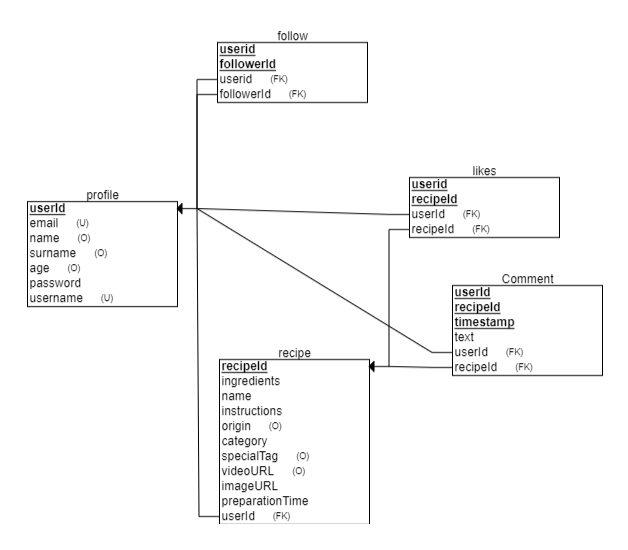
\includegraphics[width=1\linewidth]{slike/DBdiagram.png}
			    \caption{Dijagram baze podataka}
			    \label{fig:enter-label}
			\end{figure}
			
			\eject
			
			
		\section{Dijagram razreda}
	\noindent U nastavku su prikazani i opisani razredni dijagrami trenutne implementacije prilikom 2. predaje dokumentacije. Podijeljeni su u 3 dijagrama radi preglednosti, a svaki opisuje posebni sloj u arhitekturi software-a.
	\newline
	\newline		
\noindent\textbf{Controller} je sloj softvera koji upravlja dolaznim zahtjevima, obrađuje ih i koordinira tijekom izvođenja programa. Njegove klase su kontroleri (\textit{CommentController}, \textit{FollowController}, \textit{LikeController}, \textit{ProfileController} i \textit{RecipeController}) koji koordiniraju različite zahtjeve i usmjeravaju ih prema odabranim service klasama (\textit{CommentService}, \textit{FollowService}, \textit{LikeService}, \textit{ProfileService} i \textit{RecipeService}). \textit{Controller} klase su sa service klasama vezane asocijacijom, a obje ovise o osnovnim model klasama (\textit{Comment}, \textit{Follow}, \textit{Like}, \textit{Profile} i \textit{Recipe}).

\begin{figure}[H]
			    \centering
			    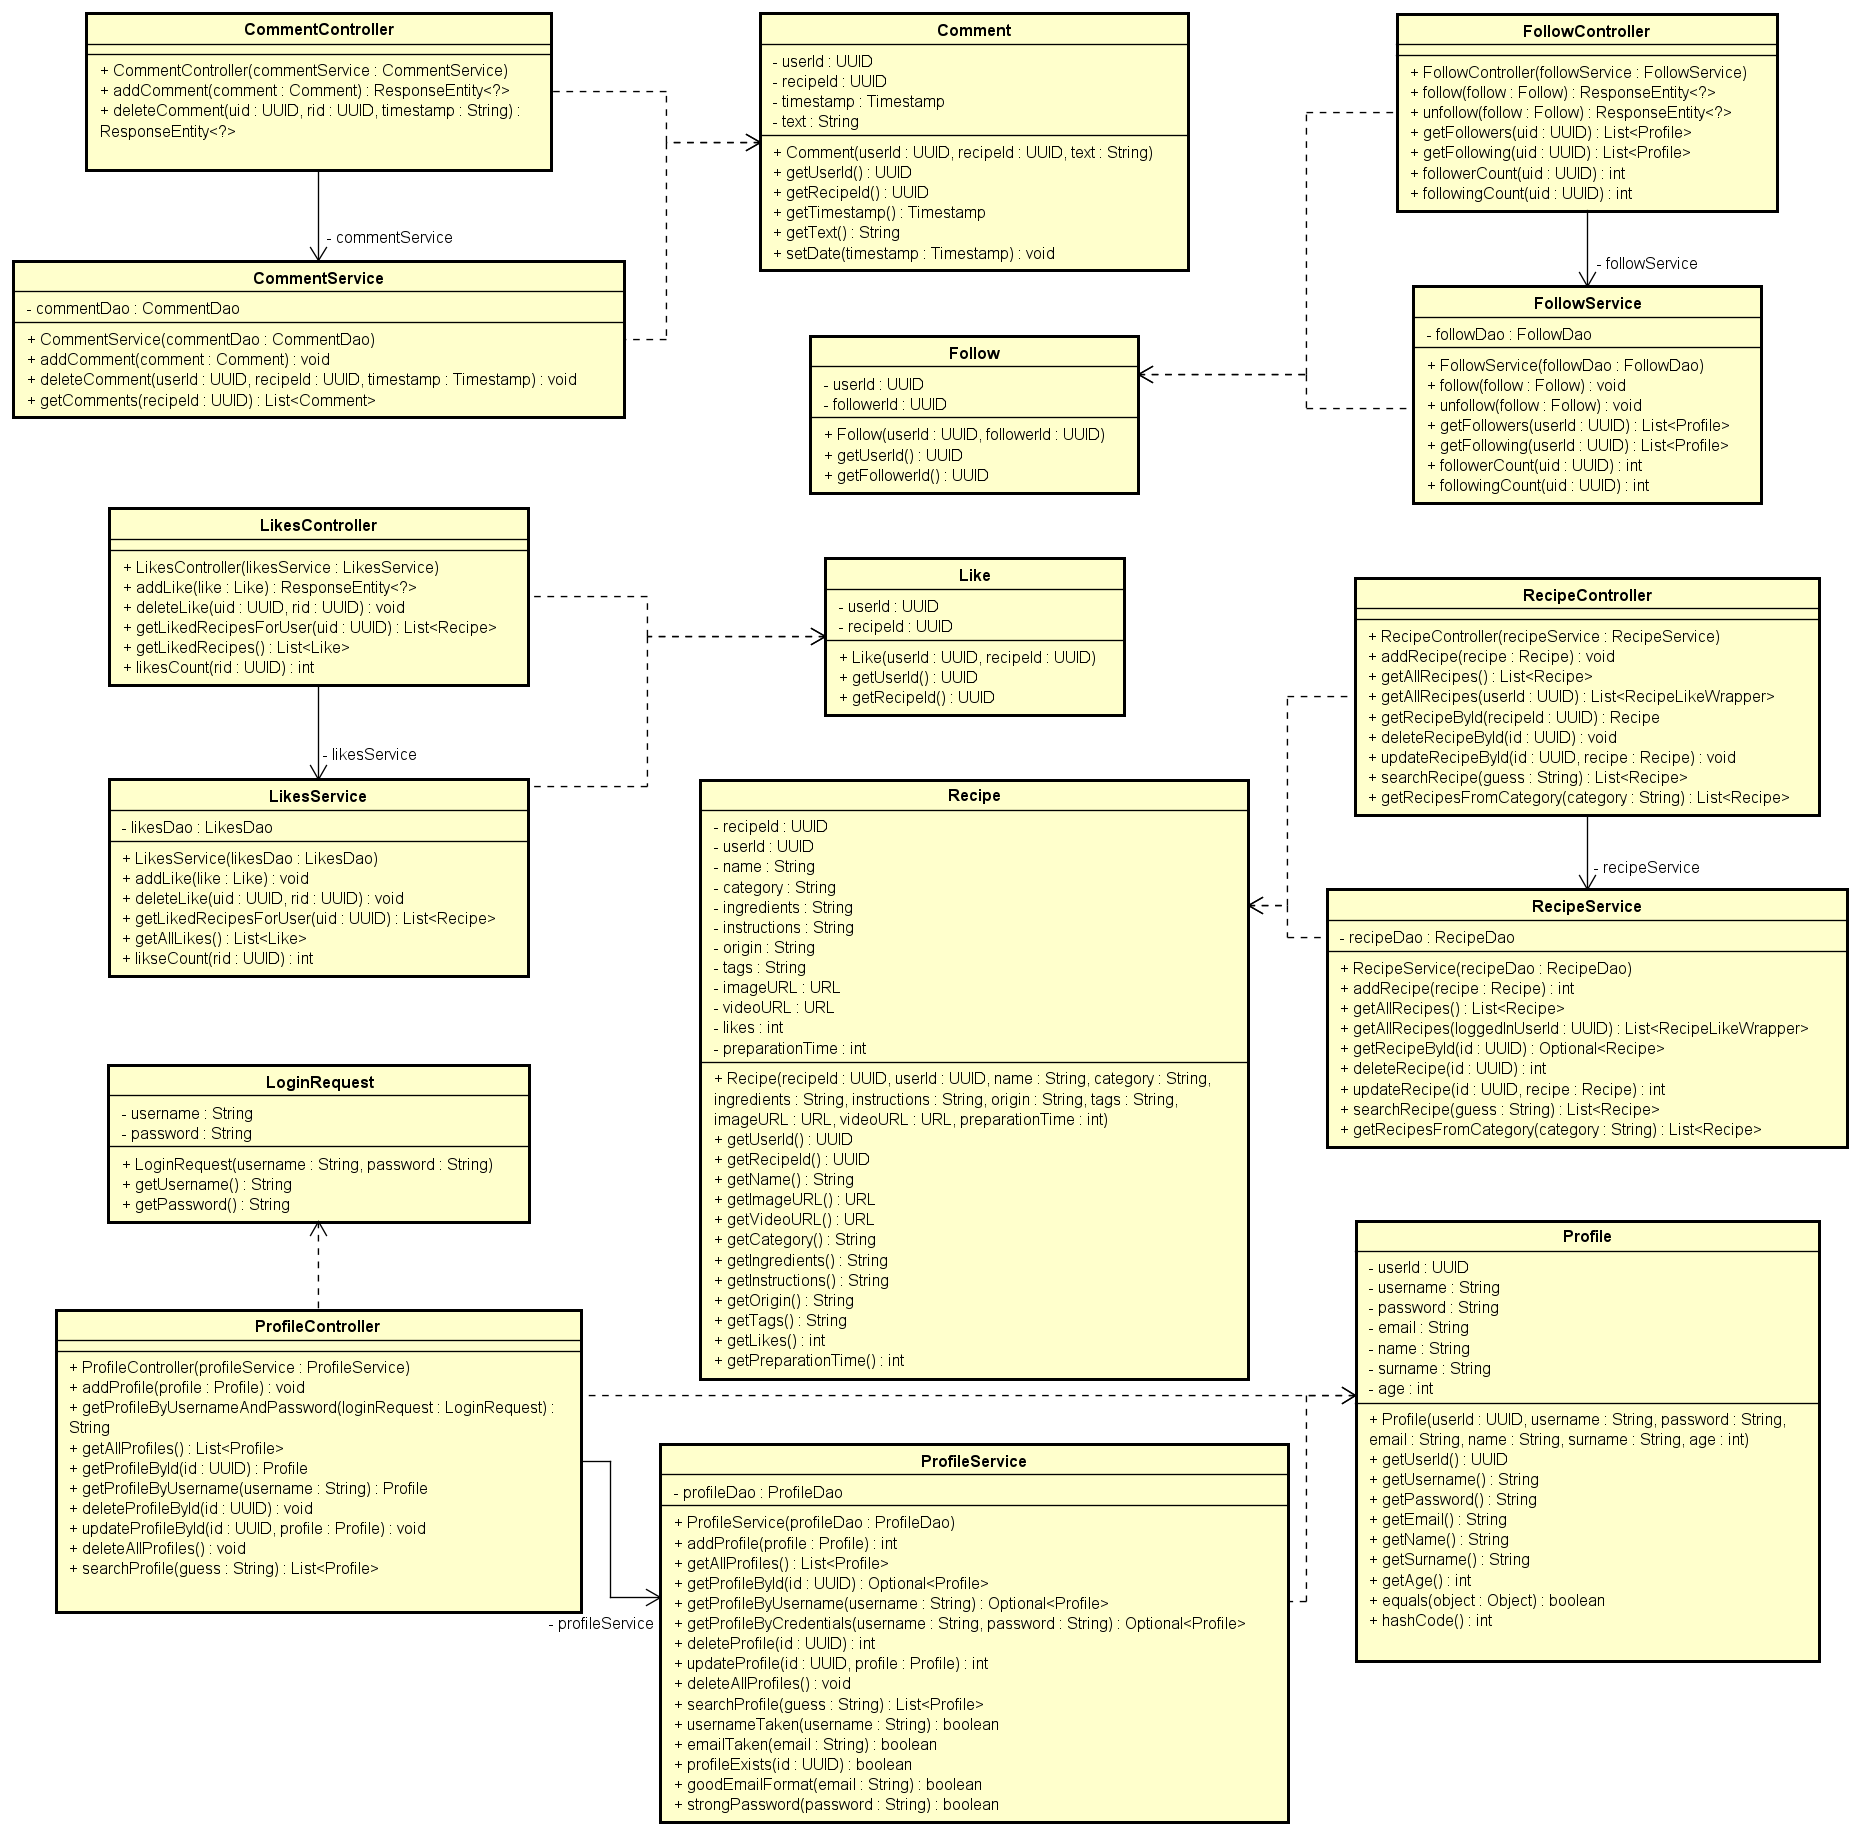
\includegraphics[width=1\linewidth]{slike//dijagrami/Controller.png}
			    \caption{Dijagram razreda - Controller}
			    \label{fig:enter-label}
			\end{figure}
	\eject		
 \noindent \textbf{Service} je sloj softvera koji pruža sučelje između kontrolera i sloja pristupa podacima. Service klase (\textit{CommentService}, \textit{FollowService}, \textit{LikeService}, \textit{ProfileService} i \textit{RecipeService}) asociraju se sa sučeljem (\textit{CommentDao}, \textit{FollowDao}, \textit{LikesDao}, \textit{ProfileDao} i \textit{RecipeDao}) preko kojeg pristupaju traženim podacima i upravljaju njima pa stoga ovise o model razredima (\textit{Comment}, \textit{Follow}, \textit{Like}, \textit{Profile} i \textit{Recipe}). U \textit{service} sloju nalaze se još klase \textit{LoginRequest} i \textit{RestExceptionHandler} koje ne pristupaju podacima direktno nego su zadužene za druge funkcionalnosti Service sloja.
 
   \begin{figure}[H]
	\centering
	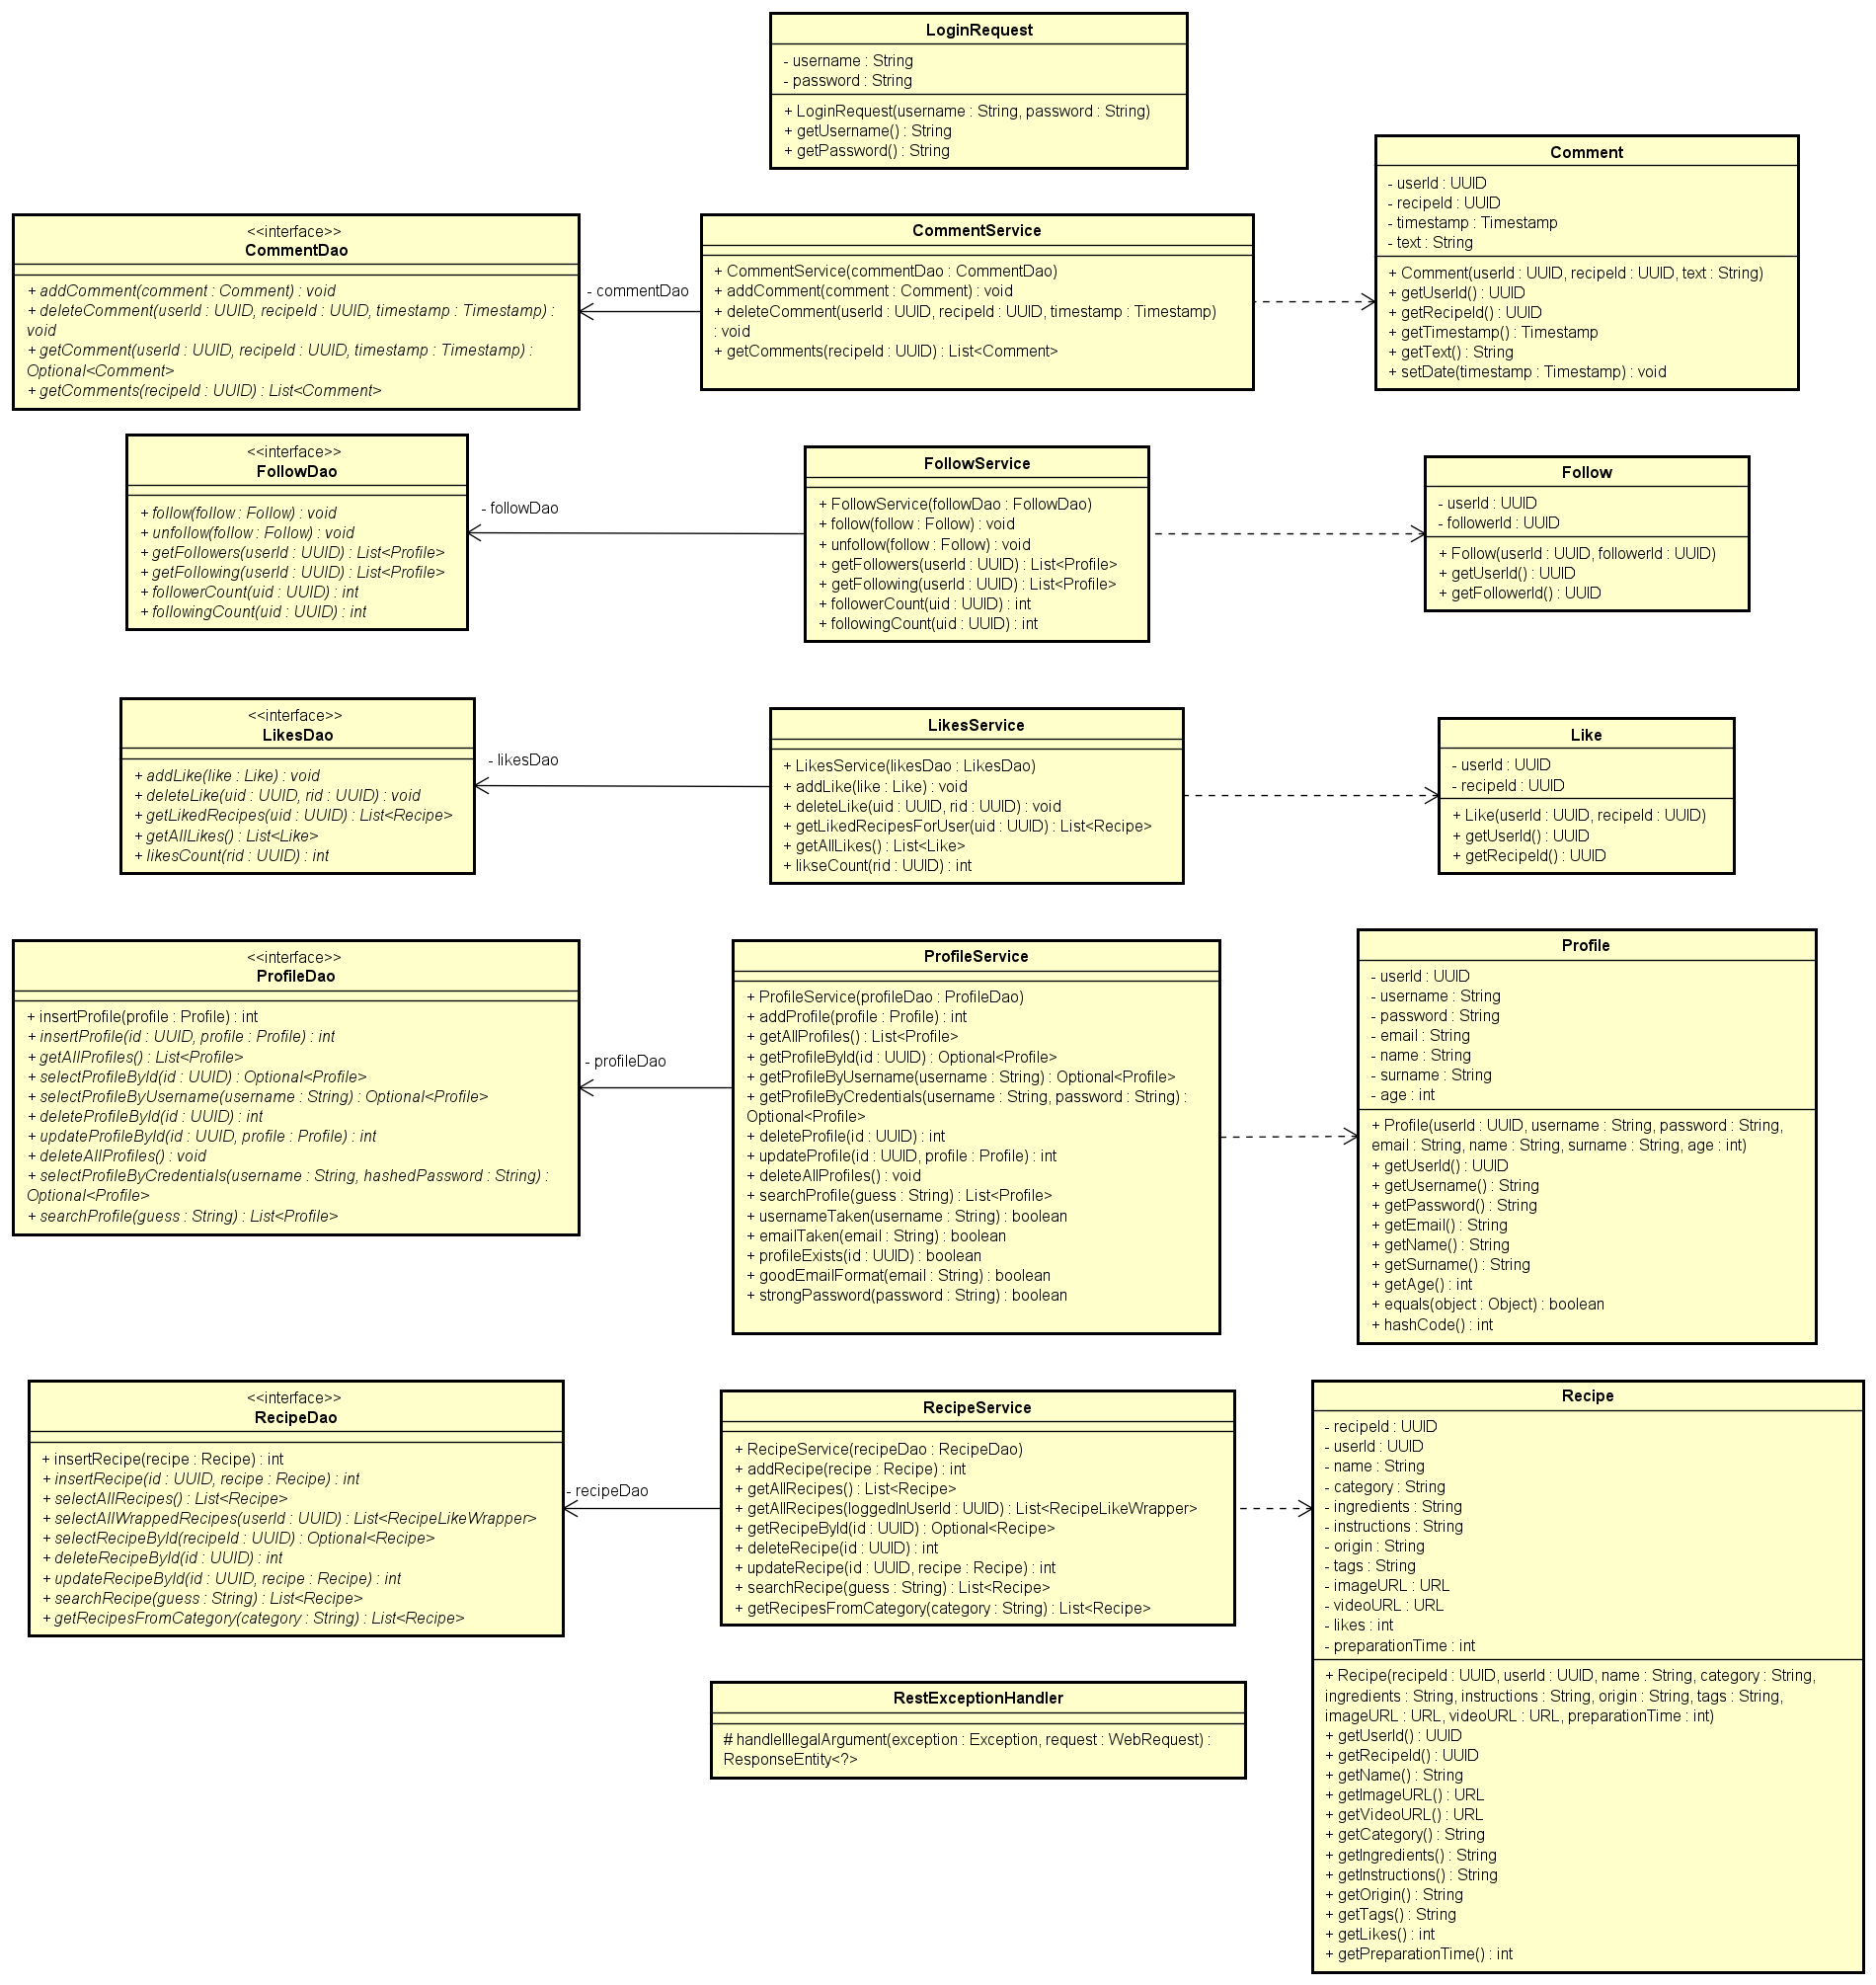
\includegraphics[width=1\linewidth]{slike/dijagrami/Service.png}
	\caption{Dijagram razreda - Service}
	\label{fig:enter-label}
\end{figure}
\eject
\noindent \textbf{DAO} (Data Access Object) predstavlja objekt koji pruža sučelje za izvođenje osnovnih operacija pristupa podacima, dodavanja, čitanja, ažuriranja i brisanja. Unutar projekta koristili smo 5 DAO sučelja (\textit{CommentDao}, \textit{FollowDao}, \textit{LikesDao}, \textit{ProfileDao} i \textit{RecipeDao}) te njihove implementacije u obliku service klasa (\textit{CommentDataAccessService}, \textit{FollowDataAccessService}, \textit{LikesDataAccessService}, \textit{ProfileDataAccessService} i \textit{RecipeDataAccessService}) s omogućenim pristupom podacima. Uz to, implementirane klase asocijacijom su vezane na klasu \textit{JdbcTemplate} radi formatiranja u svrhu jednostavnije implementacije.

\begin{figure}[H]
	\centering
	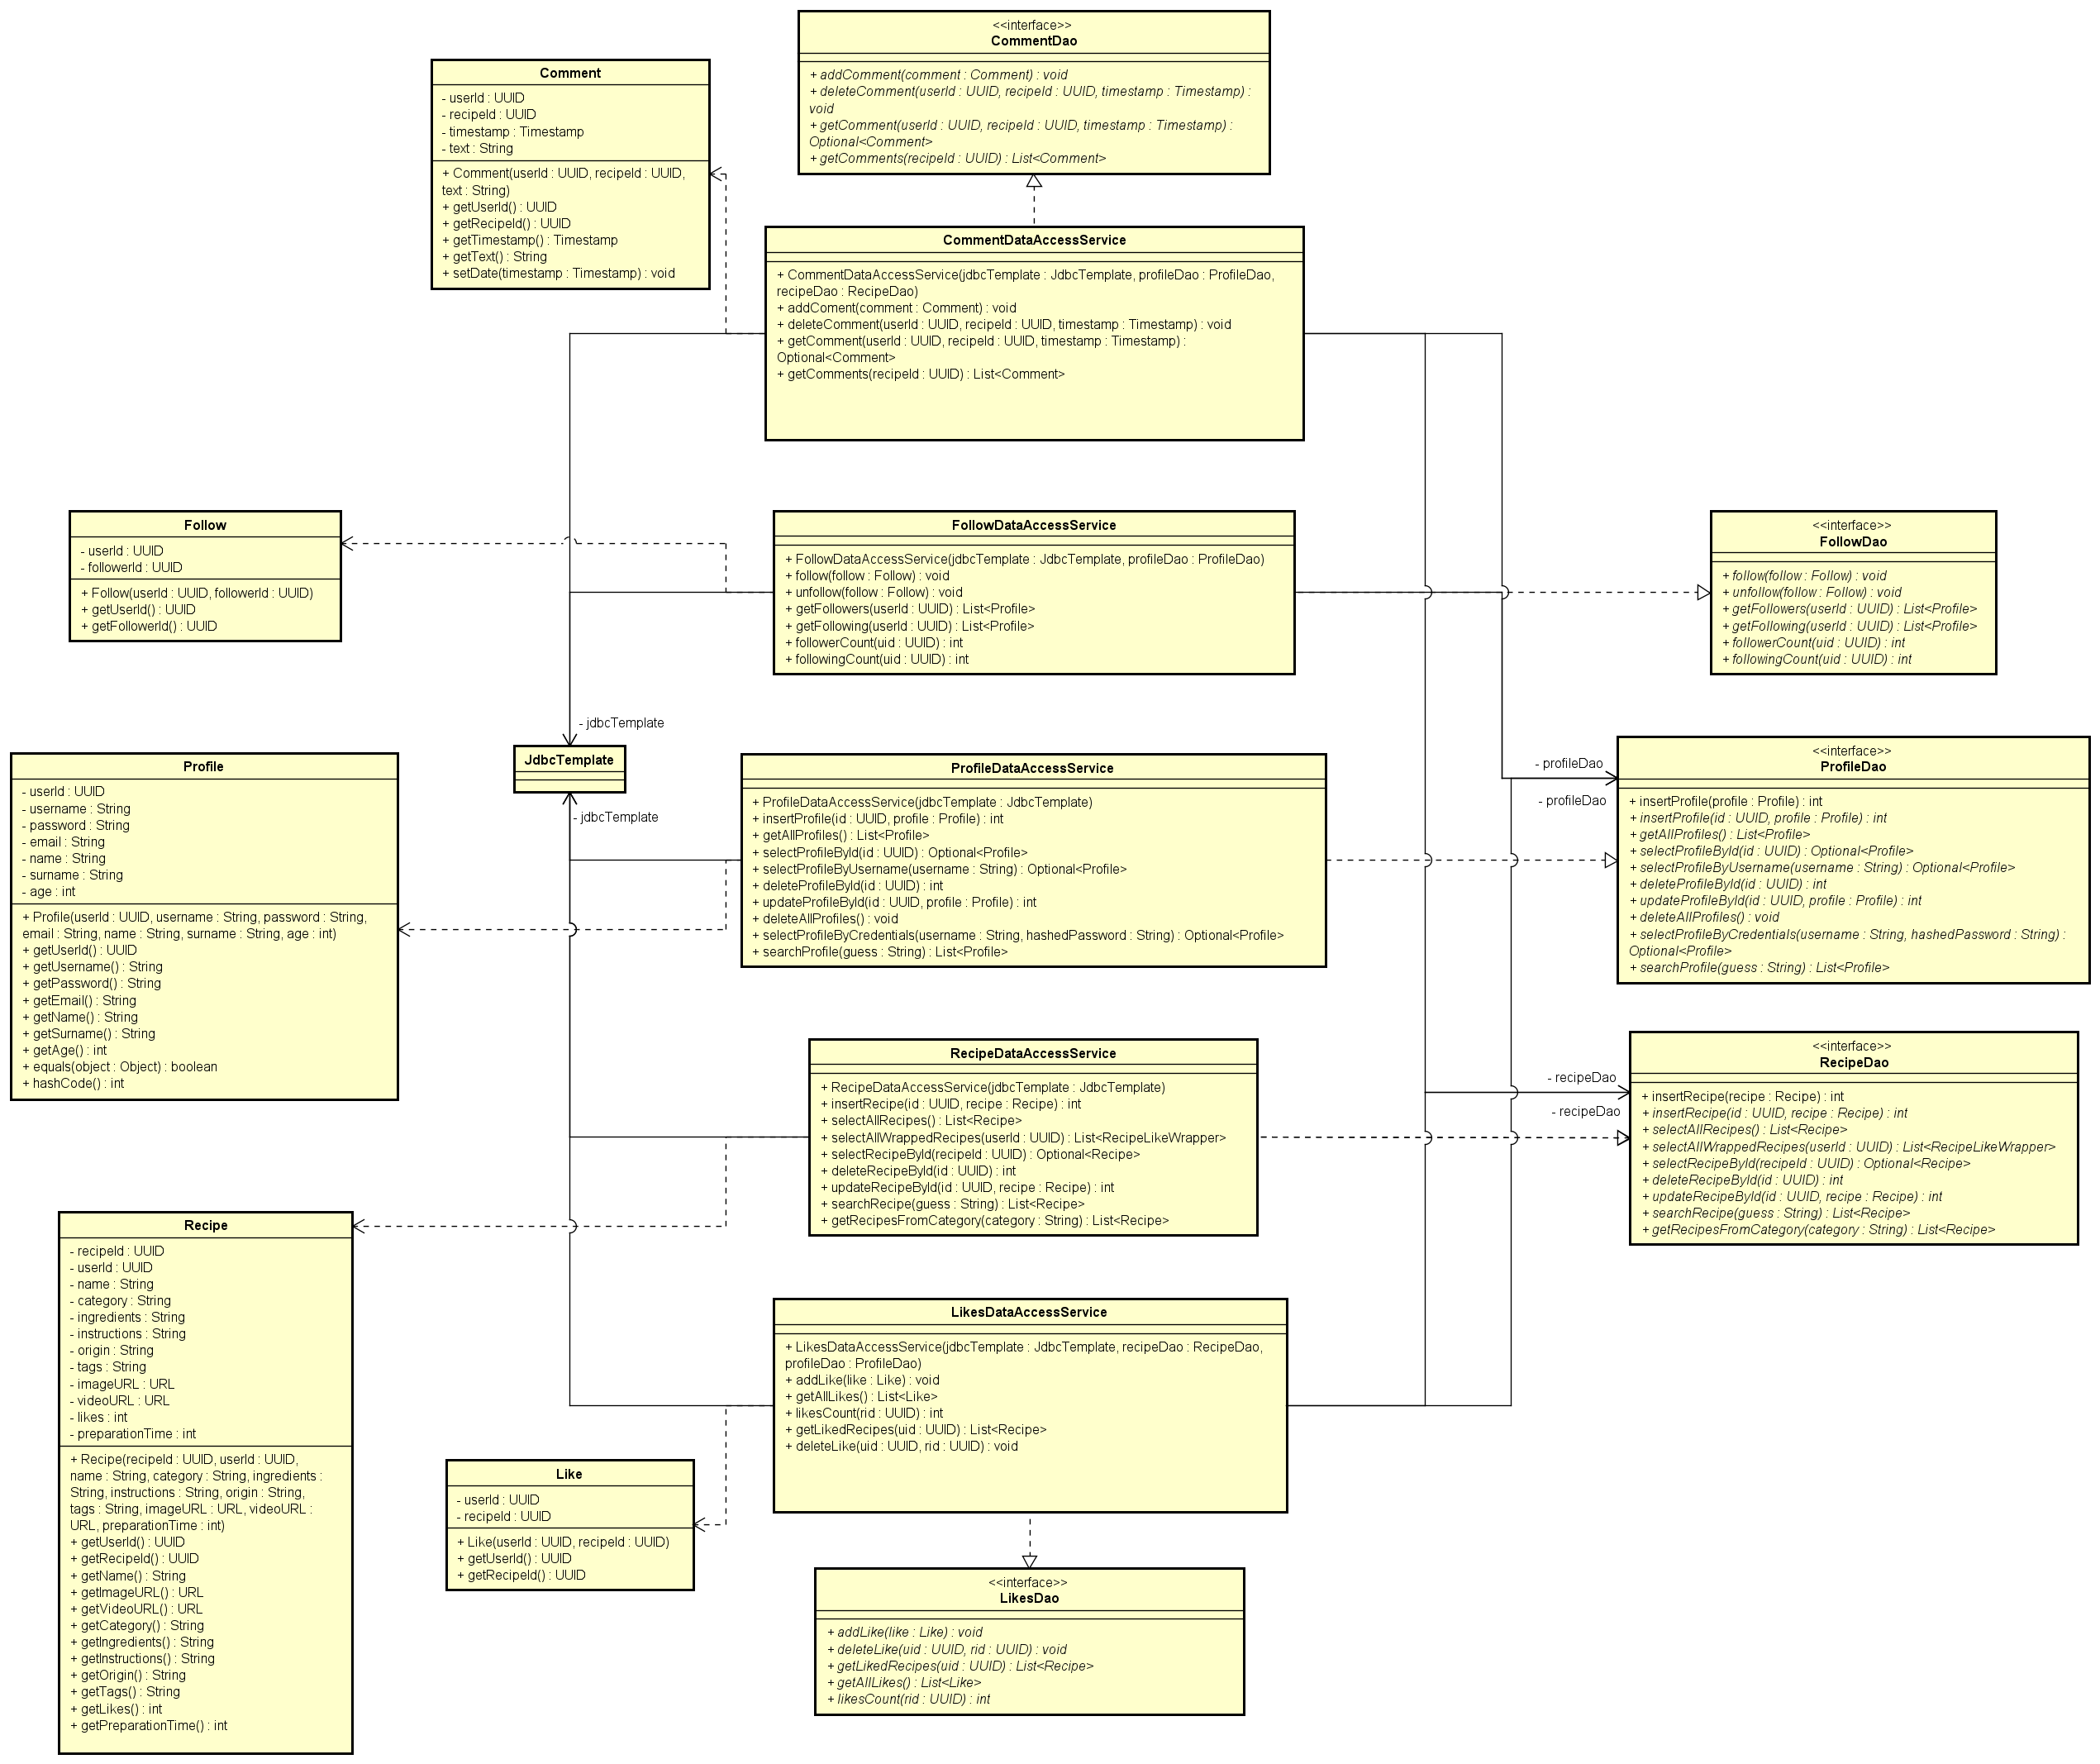
\includegraphics[width=1\linewidth]{slike/dijagrami/Dao.png}
	\caption{Dijagram razreda - Dao}
	\label{fig:enter-label}
\end{figure}
\eject
%    \textbf{\textit{dio 2. revizije}}\\			
			
% 			\textit{Prilikom druge predaje projekta dijagram razreda i opisi moraju odgovarati stvarnom stanju implementacije}
			
			
			
% 			\eject
		
		\section{Dijagram stanja}

		\noindent Dijagram stanja prikazuje stanja prijavljenog i neprijavljenog korisnika. Korisnik inicijalno nije prijavljen. Neprijavljeni korisnik iz home pagea ima opciju stisnuti gumb za pretraživanje novih recepata ili pregledavati recepte (ako ih ima) temeljem kategorija (npr. predjela, deserti), vrsta kuhinje (talijanska, kineska) ili specifičnih sastojaka uz pomoć tražilice. Neprijavljeni korisnik također može potražiti autora recepta temeljem korisničkog imena putem tražilice. Za pristup svim ostalim mogućnostima platforme, korisnik se mora registrirati ili prijaviti. Prijavljeni korisnik može sve što i neprijavljeni korisnik, a može koristiti i još neke stvari. Može stisnuti za gumb za dodavanje vlastitog recepta ili na gumb za pregled svih recepata koje je spremio. Također je moguće i pregledati te uređivati vlastiti profil na stranici profila. Još jedna pogodnost koju prijavljeni korisnici imaju je ta da mogu komunicirati s autorima putem chata ili videopoziva. Naravno, korisnik u bilo kojem trenutku može stisnuti na gumb s logoim stranice kako bi se vratio na Home page. 

		\eject
			
			\begin{figure}[H]
				\centering
				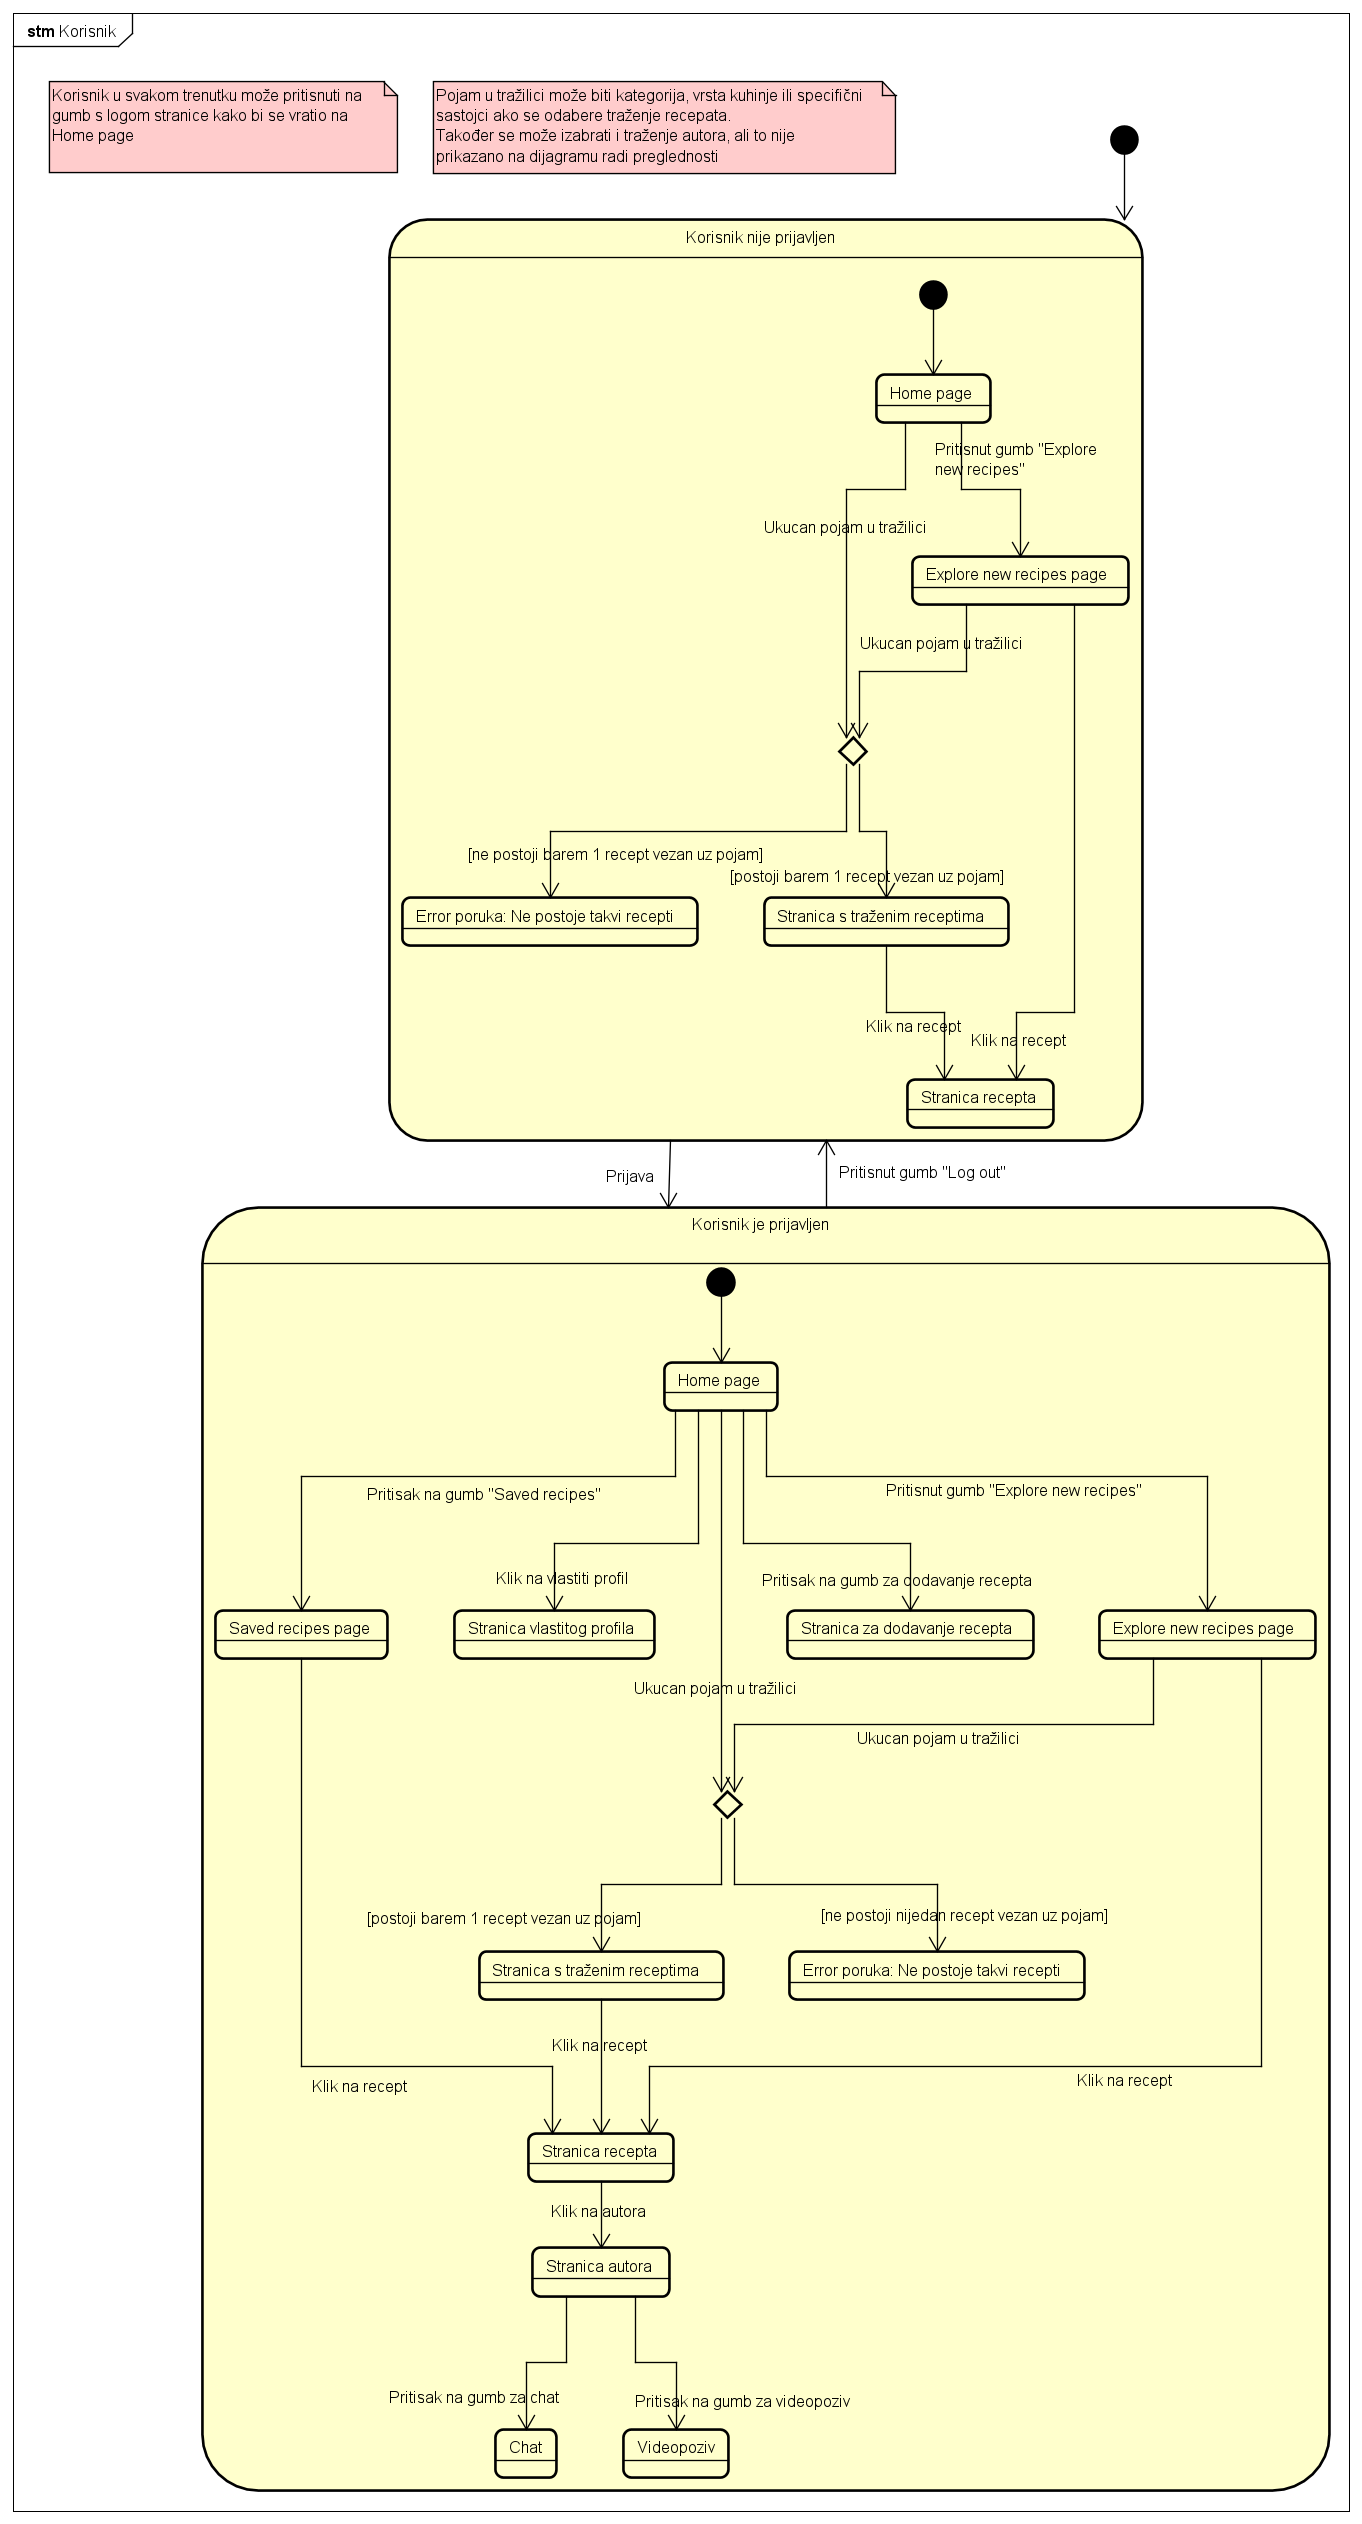
\includegraphics[height=0.95\textheight]{slike/dijagrami/Korisnik_dijagram_stanja.png}
				\caption{Dijagram stanja za korisnika}
				\label{fig:enter-label}
			\end{figure}
			
			
			\eject 
		
		\section{Dijagram aktivnosti}
			
		\noindent Dijagram aktivnosti prikazuje aktivnosti pregledavanja nespremljenih recepata i autora. Korisnik može naći nove recepte uz pomoć gumba "Explore new recipes" ili uz pomoć pretraživanja pojmova u tražilici. Kada korisnik odabere jednu od ovih dviju opcija, web aplikacija šalje upit za dohvat tih recepata bazi podataka koja daje odgovor o tome postoje li podaci i ako da, onda ih vraća. Nakon toga aplikacija prikazuje recepte na koje korisnik može kliknuti kako bi ih pohranio ili kako bi ih detaljnije pregledao. Naravno, u oba slučaja aplikacija mora slati upit bazi podataka kako bi dohvatila / pohranila podatke. Osim toga, korisnik u tražilici može pretraživati i autore pa tada baza dohvaća podatke iz tablice profiles. Nakon dohvaćanja autora, aplikacija prikazuje njegovu stranicu koja sadrži njegove podatke i recepte koje korisnik opet može pregledati i pohraniti.   

		\eject
			
			\begin{figure}[H]
				\centering
				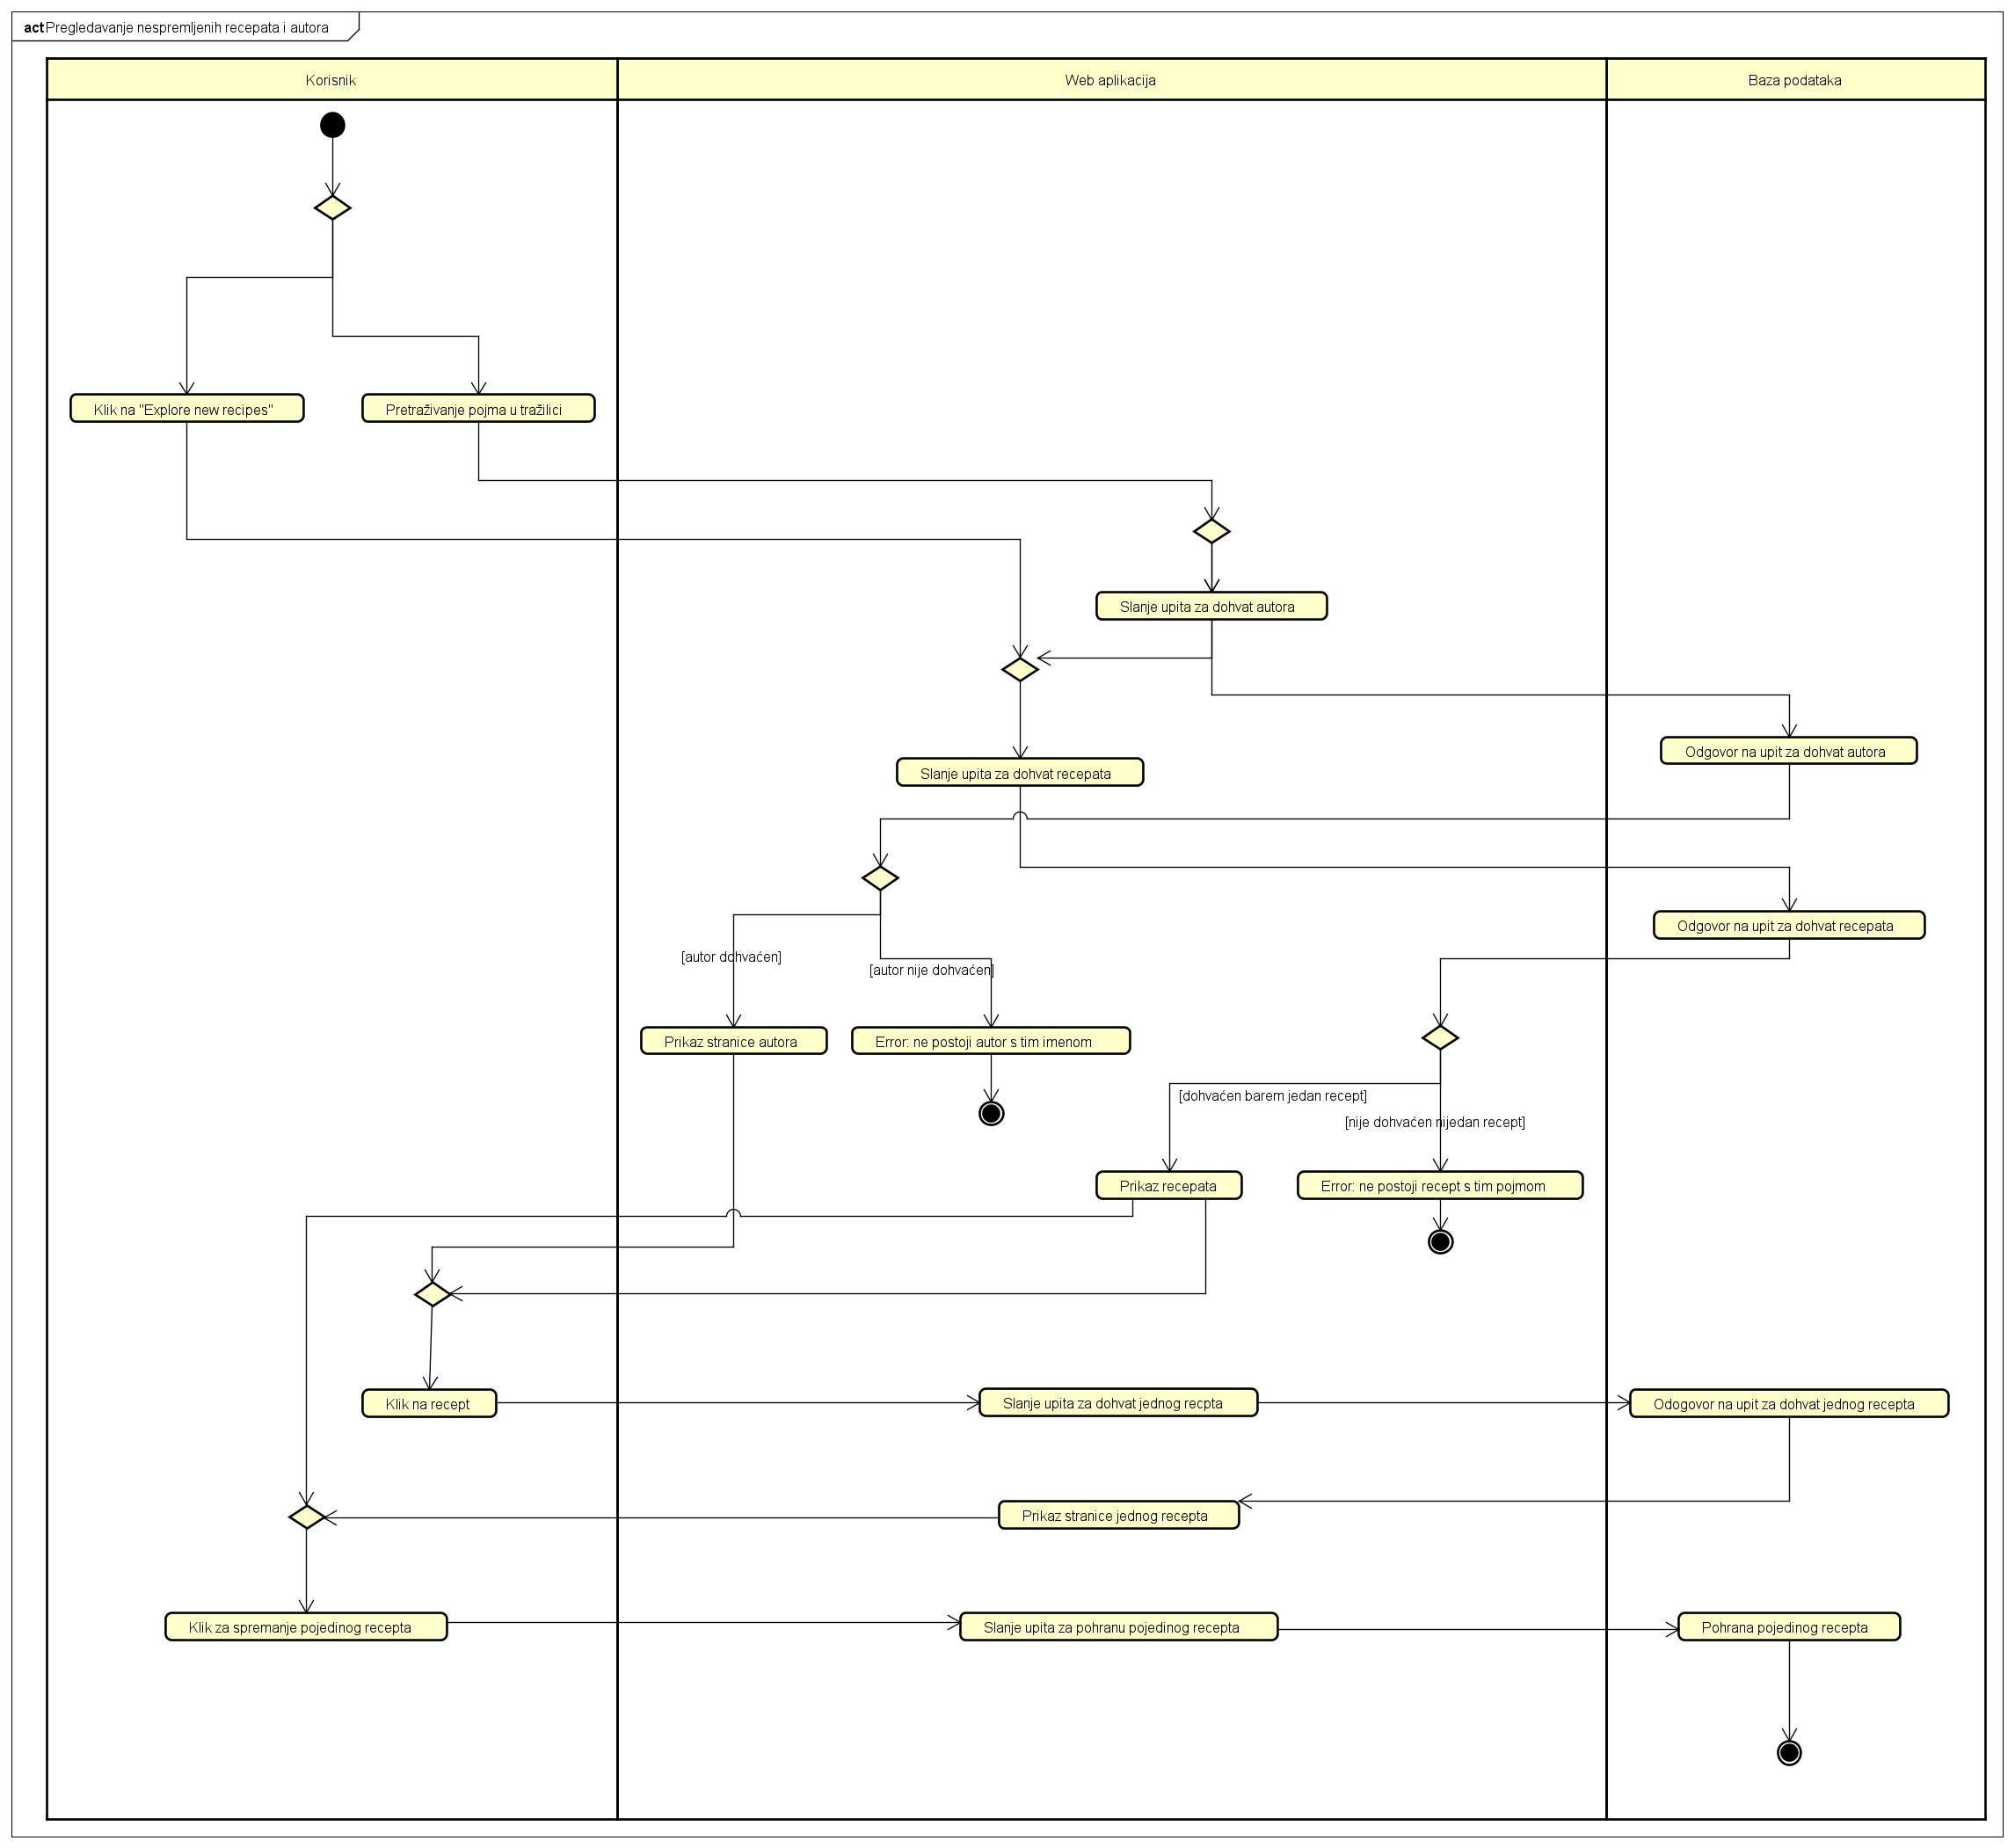
\includegraphics[width=1\textwidth]{slike/dijagrami/Pregledavanje nespremljenih recepata i autora_dijagram_aktivnosti.png}
				\caption{Dijagram aktivnosti za pregledavanje nespremljenih recepata i autora}
				\label{fig:enter-label}
			\end{figure}
			
			\eject

		\section{Dijagram komponenti}
		
		\noindent Dijagram komponenti prikazuje organizaciju i odnose komponenti koje čine programsku potporu za našu aplikaciju. Naša aplikacija koristi dva sučelja, jedno za dohvat JS i CSS datoteka, a druga za dohvat JSON datoteka. Preko sučelja za dohvat JS i CSS datoteka poslužuju se datoteke za frontend. Komponenta App.js poslužuje jednu od JS datoteka na sučelje. Te datoteke su logičke cjeline nazvane po svojoj funkciji (npr. home page, login, header). Sve te datoteke ovisne su o biblioteci \textit{react}. Preko sučelja za dohvat JSON datoteka dobivamo pristup REST API komponenti. REST API koristi HTTP zahtjeve kako bi pristupio podacima na backendu. JPA repozitorij dohvaća podatke iz baze podataka koristeći SQL upite. Komponenta React view ovisno o korisnikovim unosima prikazuje stvari s frontenda i dohvaća podatke s backenda.
			
			\begin{figure}[H]
				\centering
				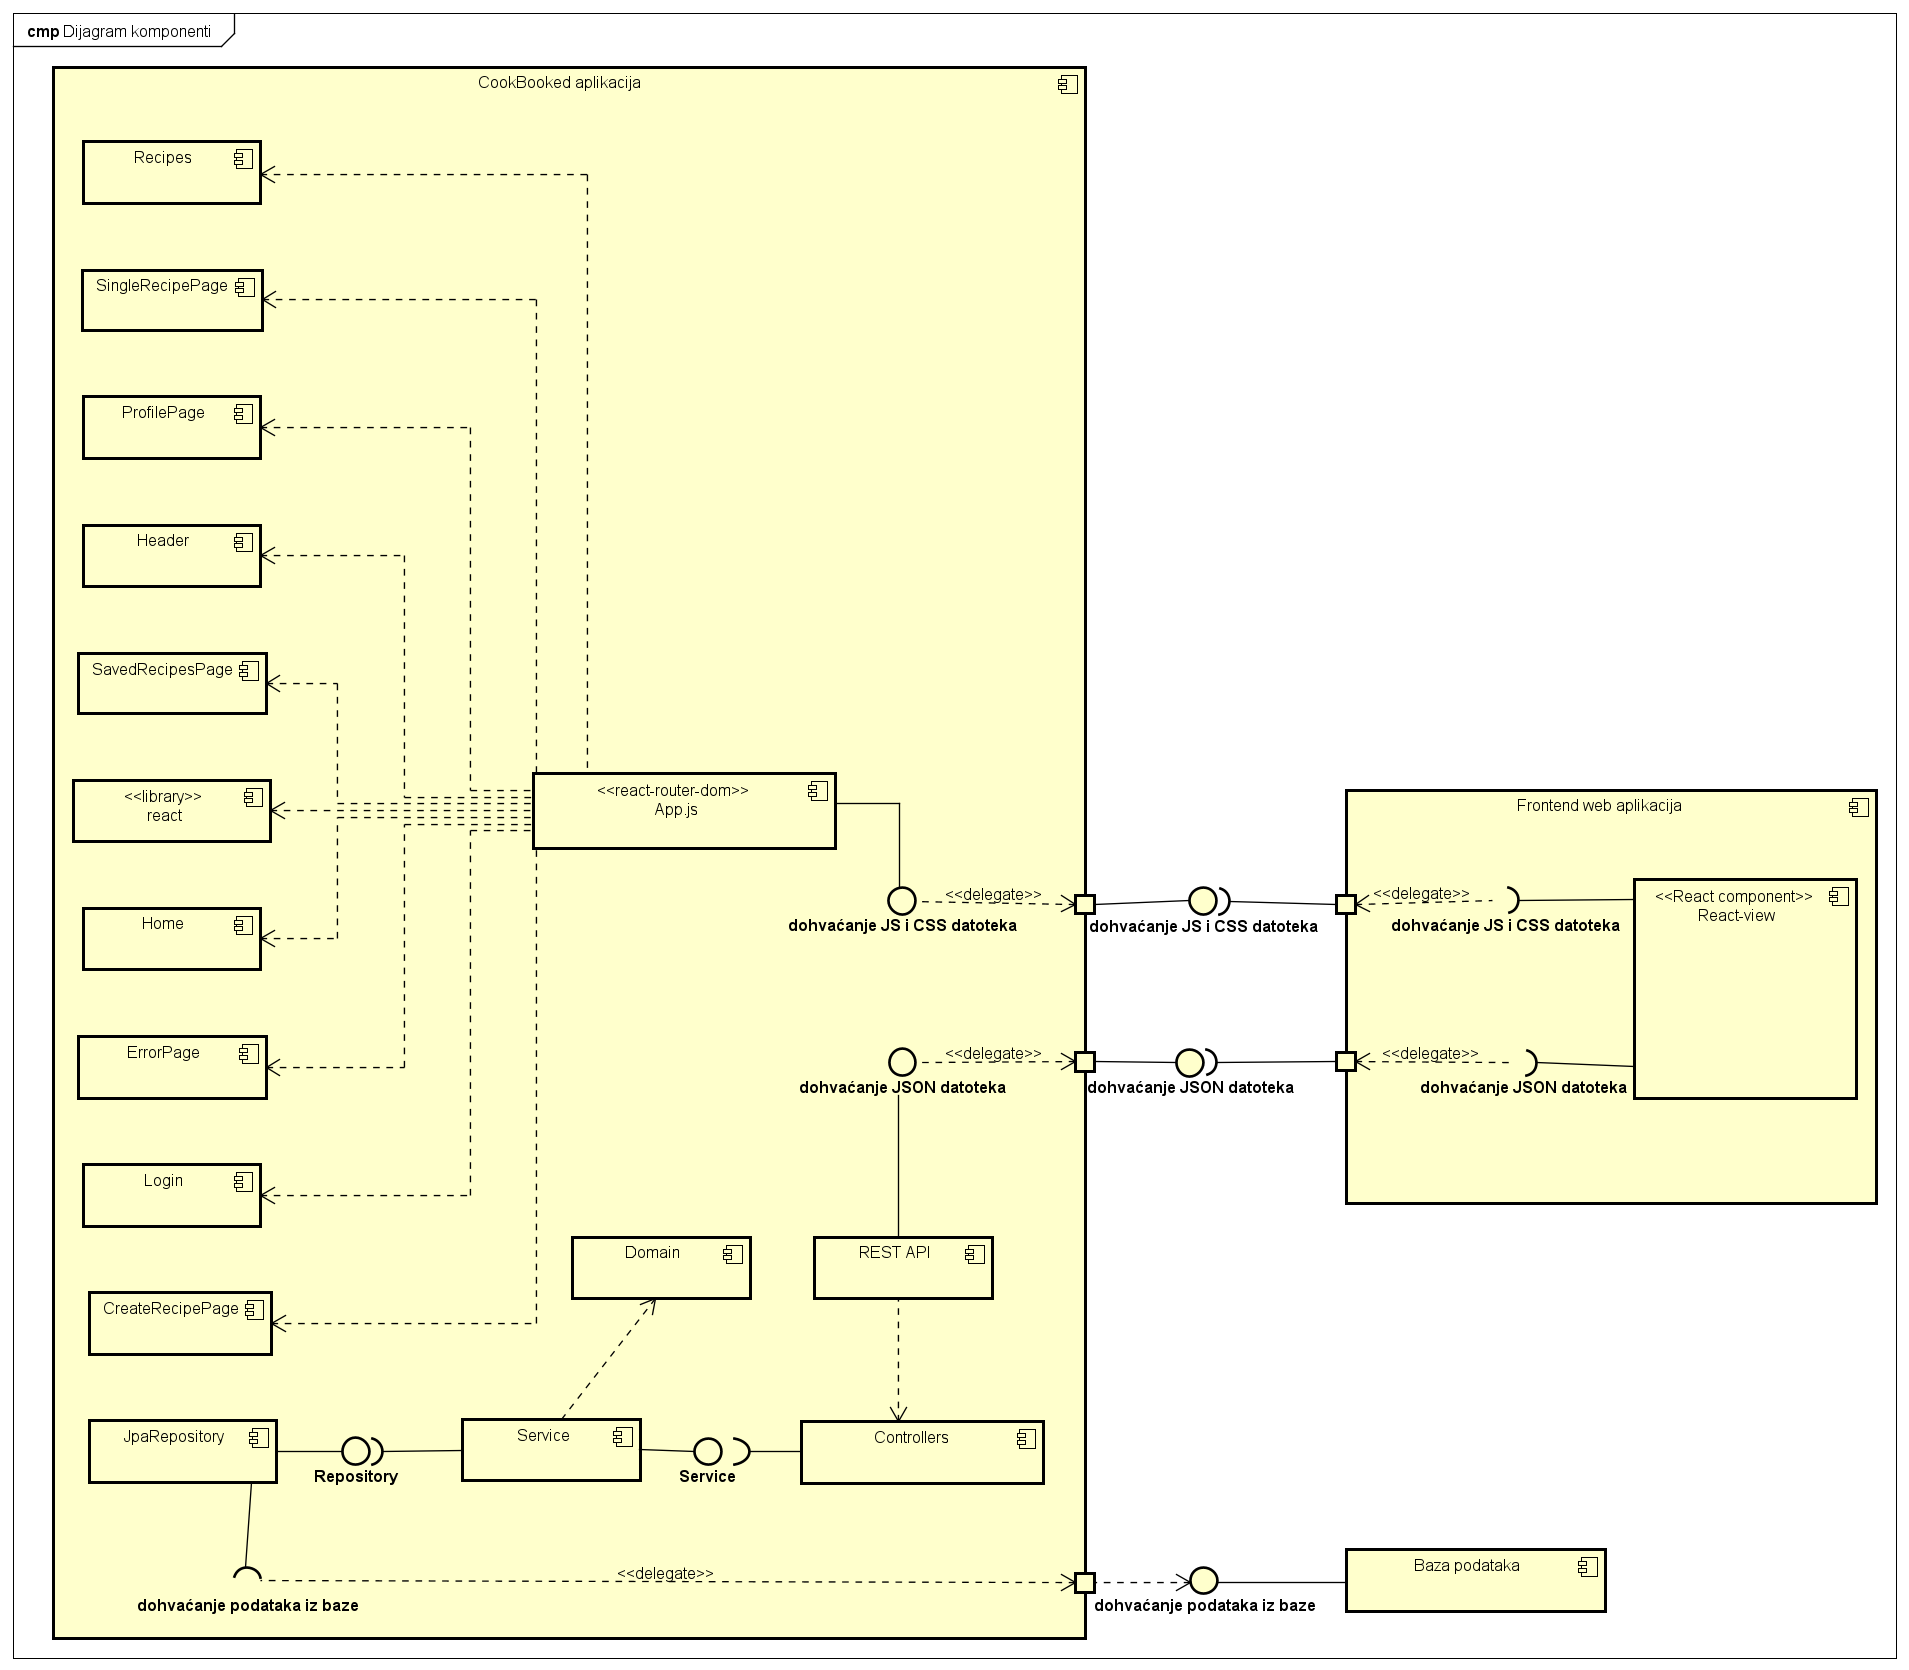
\includegraphics[width=0.95\textwidth]{slike/dijagrami/Dijagram komponenti.png}
				\caption{Dijagram komponenti}
				\label{fig:enter-label}
			\end{figure}